\section*{1D 系統架構}

\subsection*{設計理念}

我們以鋼球平衡台作為專題的主體,然後寫程式驅動雷射測距感測器當鋼球遠離時platfor,當鋼球靠近時platform放下,重複此動作直至鋼球平衡台平衡。

\begin{figure}[h!]
    \centering
    \begin{minipage}[b]{0.45\textwidth}
        \centering
        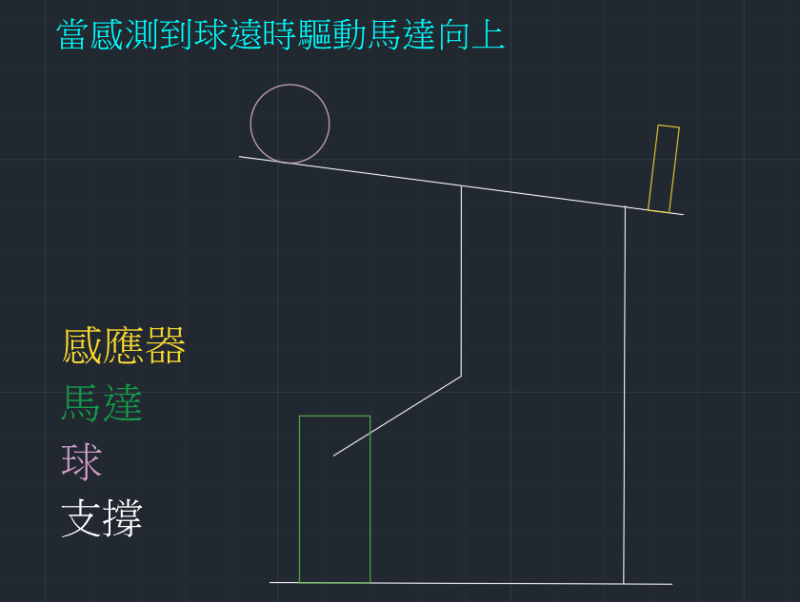
\includegraphics[width=\textwidth,height=0.22\textheight]{./../images/螢幕擷取畫面 2024-05-22 181158.png}
        \caption{2D草圖(1)}
    \end{minipage}
    \hfill
    \begin{minipage}[b]{0.45\textwidth}
        \centering
        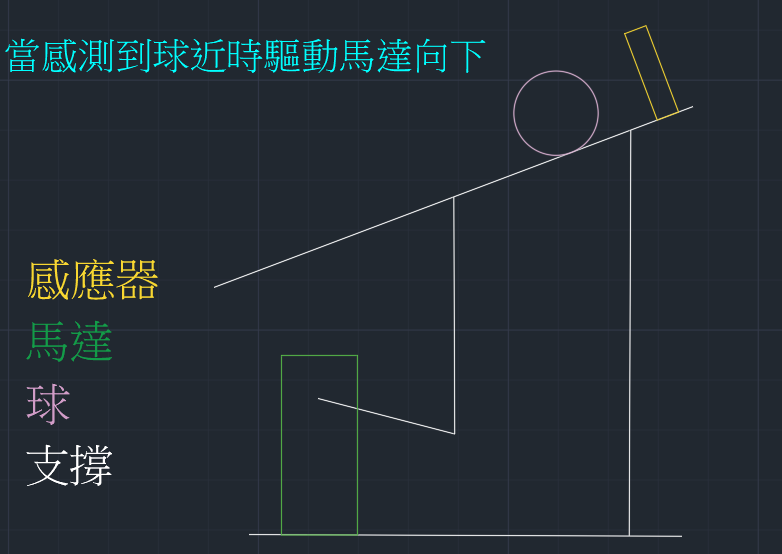
\includegraphics[width=\textwidth,height=0.22\textheight]{./../images/螢幕擷取畫面 2024-05-22 180925.png} 
        \caption{2D草圖(2)}
    \end{minipage}
\end{figure}

\subsection*{馬達角度所對應之平台角度關係}

\begin{figure}[htbp]
    \centering
    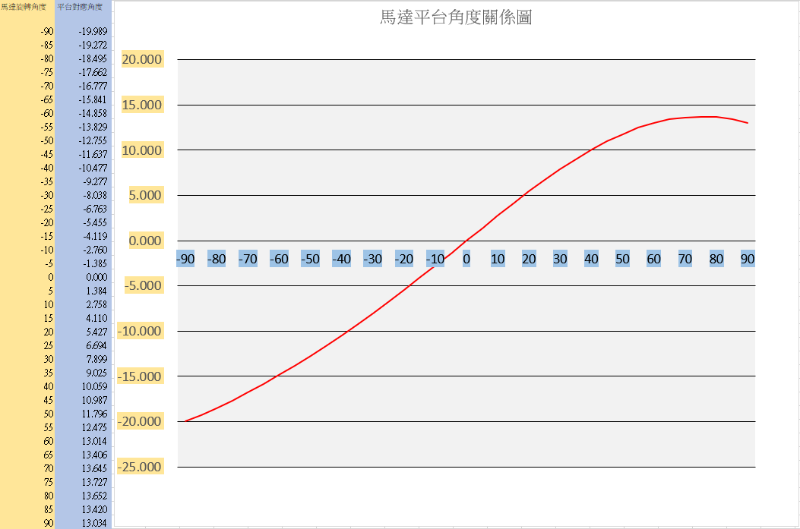
\includegraphics[width=1\textwidth]{./../images/6-1-50}
    \caption{馬達角度關係圖}
\end{figure}

\newpage

使用 SolidWorks 2023 進行繪圖。
\begin{figure}[htbp]
    \centering
    
\includegraphics[width=0.5\textwidth]{./../images/6-1-1}
    \caption{SOLIDWORKS}
\end{figure}

\subsection*{platform}

第一版本鋼球平衡台的 platform 軌道長度為 200mm 整體的寬度為 30mm 並給定深度填料 11mm。

\begin{figure}[h!]
    \centering
    \begin{minipage}[b]{0.6\textwidth}
        \centering
        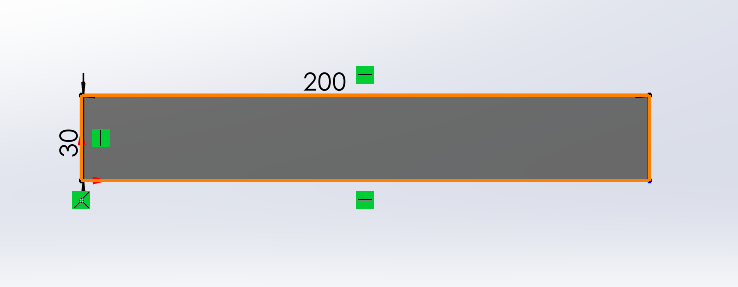
\includegraphics[width=\textwidth,height=0.22\textheight]{./../images/6-1-11}
        \caption{PLATFORM草圖 (1)}
        \label{fig:platform}
    \end{minipage}
    \hfill
    \begin{minipage}[b]{0.35\textwidth}
        \centering
        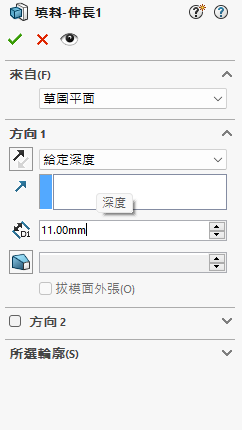
\includegraphics[width=\textwidth,height=0.25\textheight]{./../images/6-1-12} 
        \caption{編輯特徵(1)}
        \label{fig:feature1}
    \end{minipage}
\end{figure}
    
軌道上方寬度為 8.5mm,下方為 7.2mm,深 4mm並將紅圈處深伸長除料選擇完全貫穿。

\begin{figure}[h!]
    \centering
    \begin{minipage}[b]{0.6\textwidth}
        \centering
        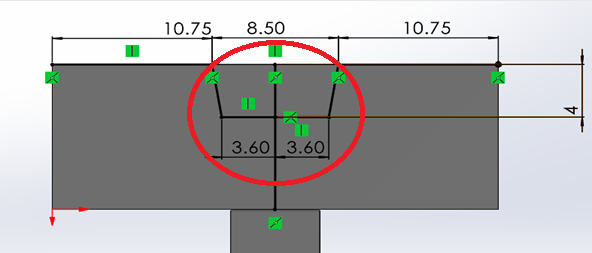
\includegraphics[width=\textwidth,height=0.22\textheight]{./../images/6-1-13}
        \caption{PLATFORM草圖 (2)}
        \label{fig:platform}
    \end{minipage}
    \hfill
    \begin{minipage}[b]{0.35\textwidth}
        \centering
        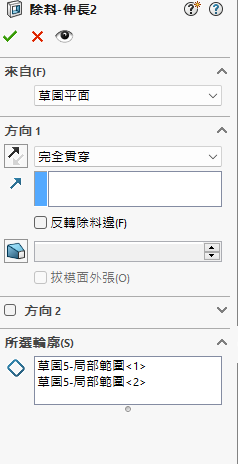
\includegraphics[width=\textwidth,height=0.25\textheight]{./../images/6-1-14} 
        \caption{編輯特徵(2)}
        \label{fig:feature1}
    \end{minipage}
\end{figure}

\newpage

下方配合處長 30mm 寬 6mm,繪製好圖形草圖。

\begin{figure}[htbp]
    \centering
    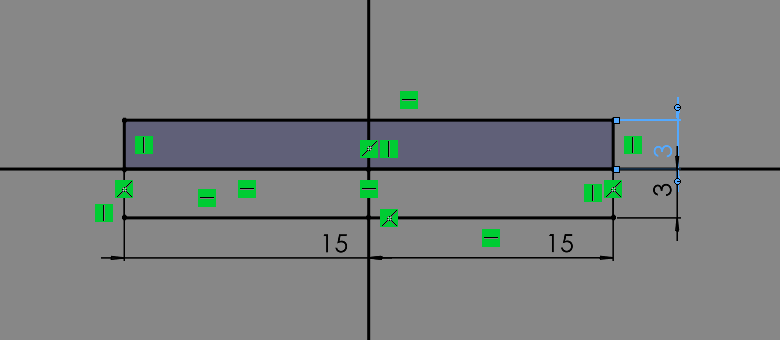
\includegraphics[width=0.7\textwidth]{./../images/6-1-15}
    \caption{PLATFORM草圖 (3)}
\end{figure}

給予尺寸後伸長填料 25mm。
\begin{figure}[h!]
    \centering
    \begin{minipage}[b]{0.6\textwidth}
        \centering
        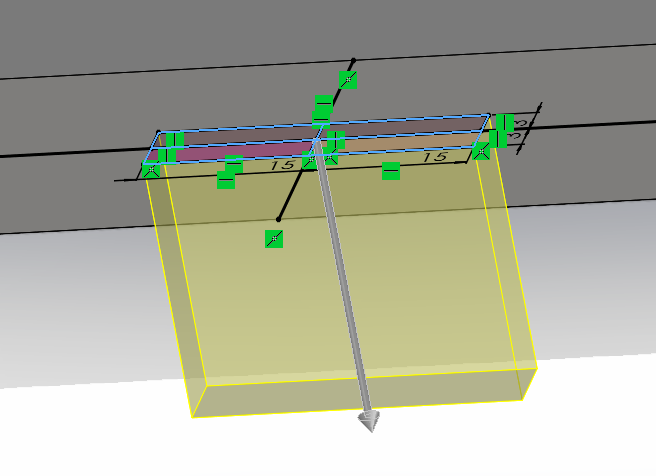
\includegraphics[width=\textwidth,height=0.22\textheight]{./../images/6-1-16}
        \caption{PLATFORM草圖 (4)}
        \label{fig:platform}
    \end{minipage}
    \hfill
    \begin{minipage}[b]{0.35\textwidth}
        \centering
        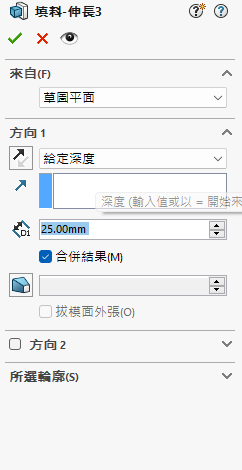
\includegraphics[width=\textwidth,height=0.25\textheight]{./../images/6-1-17} 
        \caption{編輯特徵(3)}
        \label{fig:feature1}
    \end{minipage}
\end{figure}

填料完成後再圖形上畫一個 2.9mm 的小孔並進行伸長除料以便與其他零件配合。

 \begin{figure}[htbp]
        \centering
        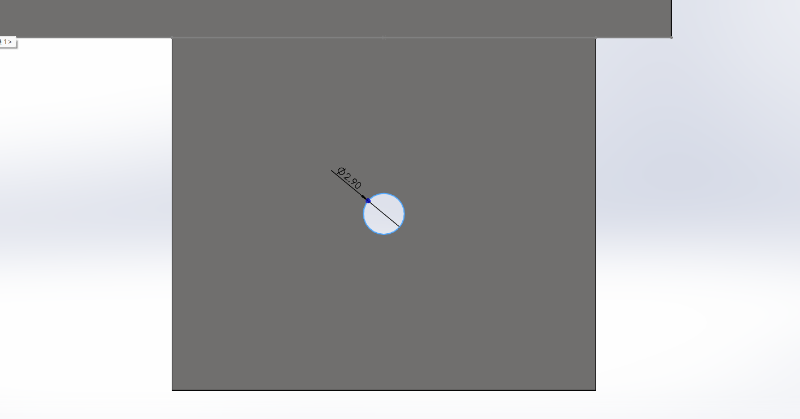
\includegraphics[width=0.49\textwidth]{./../images/6-1-18}
        \caption{PLATFORM草圖 (5)}
    \end{figure}

\newpage

第一版 platform 完成圖。

\begin{figure}[htbp]
    \centering
    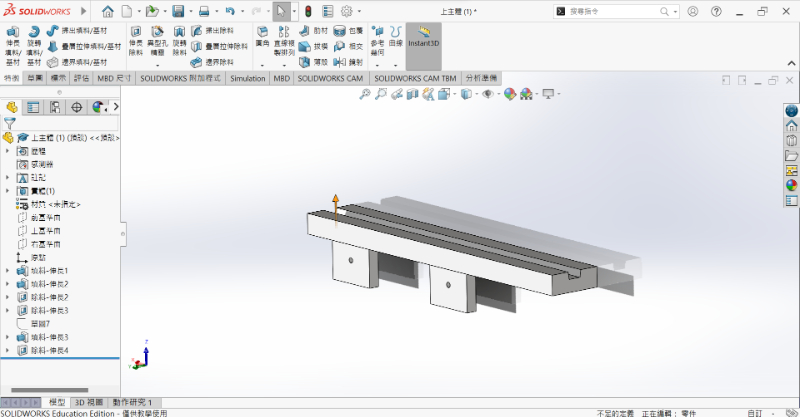
\includegraphics[width=0.78\textwidth]{./../images/6-1-19}
    \caption{PLATFORM草圖 (5)}
\end{figure}

\textbf{修改部分}

軌道上方增加長 26.2mm 寬 2mm 的貫穿凹槽,用於放置感應器。

\begin{figure}[htbp]
    \centering
    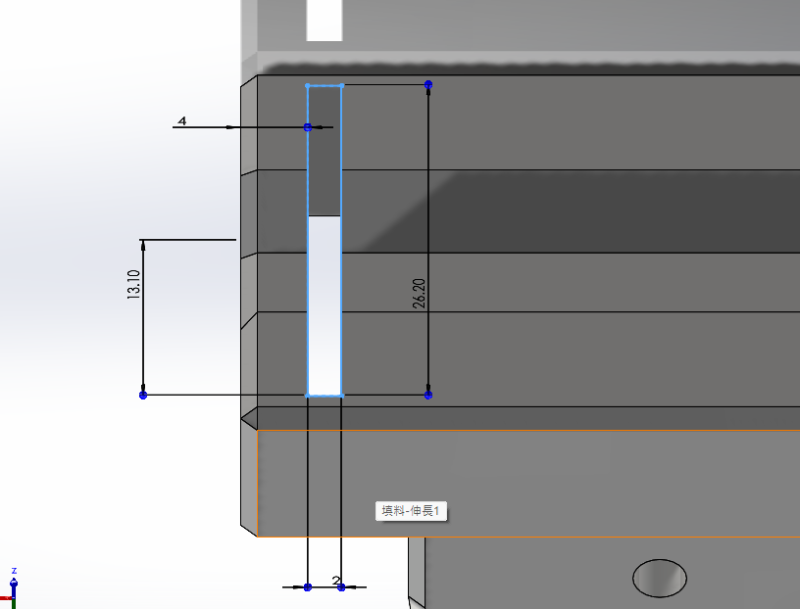
\includegraphics[width=0.42\textwidth]{./../images/6-1-20}
    \caption{修改PLATFORM草圖 (1)}
\end{figure}


下方接合處新增 R10 圓角。

\begin{figure}[htbp]
    \centering
    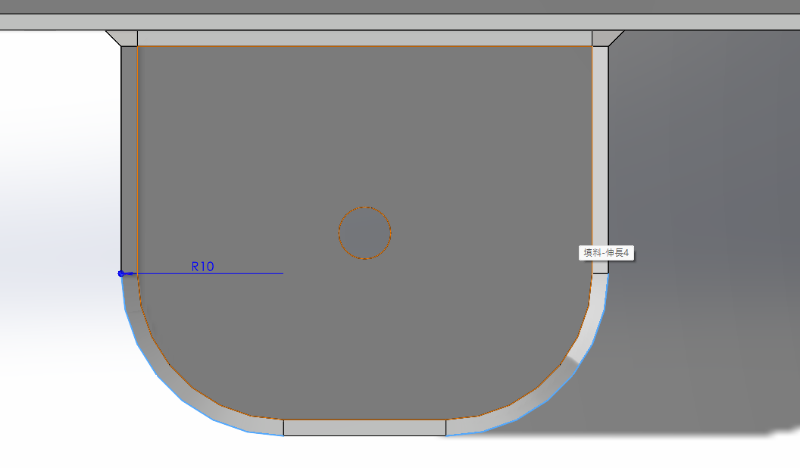
\includegraphics[width=0.4\textwidth]{./../images/6-1-21}
    \caption{修改PLATFORM草圖 (2)}
\end{figure}

\newpage


最終 Platform 零件圖。

\begin{figure}[htbp]
    \centering
    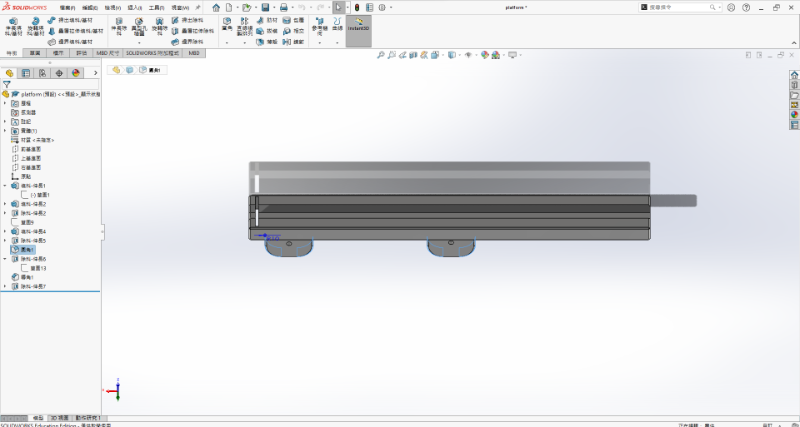
\includegraphics[width=0.9\textwidth]{./../images/6-1-22}
    \caption{最終PLATFORM零件圖}
\end{figure}

\textbf{3D 列印成果}

\begin{figure}[htbp]
    \centering
    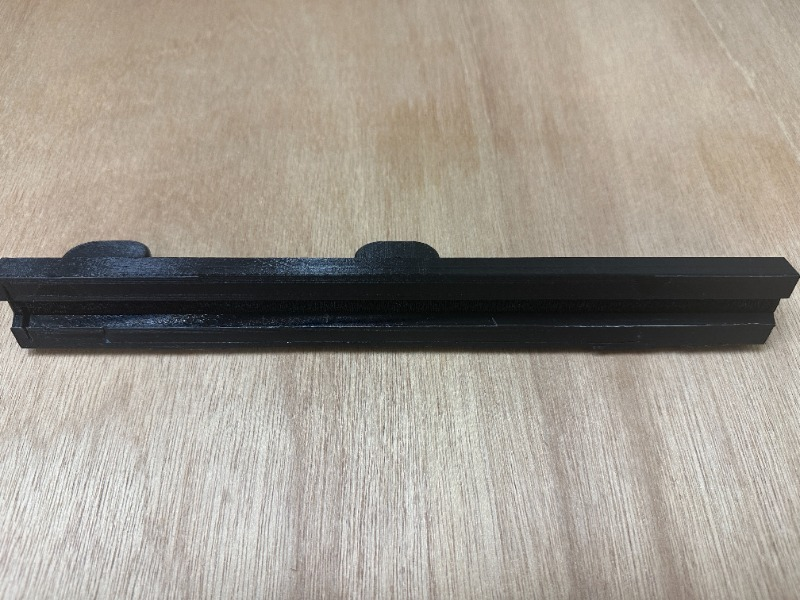
\includegraphics[width=0.8\textwidth]{./../images/6-1-26}
    \caption{PLATFORM 3D列印完成圖}
\end{figure}

\newpage

\subsection*{base}

第一版 Base 底的長為 237mm 寬為 150mm。

\begin{figure}[htbp]
    \centering
    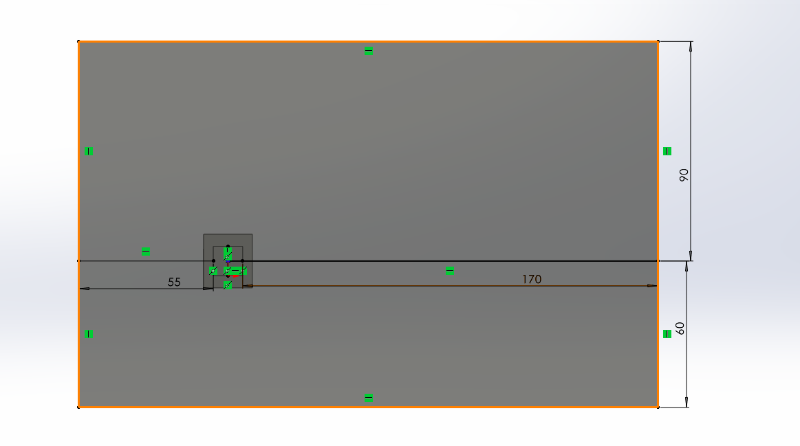
\includegraphics[width=1\textwidth]{./../images/6-1-27}
    \caption{BASE草圖(1)}
\end{figure}



在底板長 55mm 寬 54mm 處繪製一個 12mm $\times$ 12mm 的方形柱並向上填料 100mm。

\begin{figure}[h!]
    \centering
    \begin{minipage}[b]{0.6\textwidth}
        \centering
        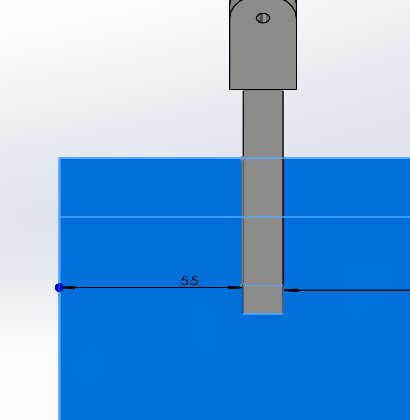
\includegraphics[width=\textwidth,height=0.35\textheight]{./../images/6-1-28}
        \caption{BASE草圖(2)}
        \label{fig:platform}
    \end{minipage}
    \hfill
    \begin{minipage}[b]{0.35\textwidth}
        \centering
        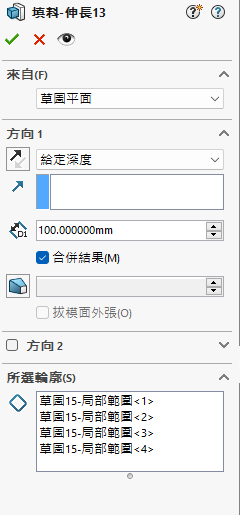
\includegraphics[width=\textwidth,height=0.35\textheight]{./../images/6-1-29} 
        \caption{編輯特徵(4)}
        \label{fig:feature1}
    \end{minipage}
\end{figure}

\newpage

在方柱上方繪製一個長 30.28mm 寬 20 的長方體然後在長方體上畫直徑 20mm 的半圓最後在圓的中心繪製一個 3.98mm 的小孔最後在長方體上畫一個長 30mm 寬 10.8mm 的小長方體伸長除料選擇完全貫穿方便與上方 platform 配合。

\begin{figure}[h!]
    \centering
    \begin{minipage}[b]{0.45\textwidth}
        \centering
        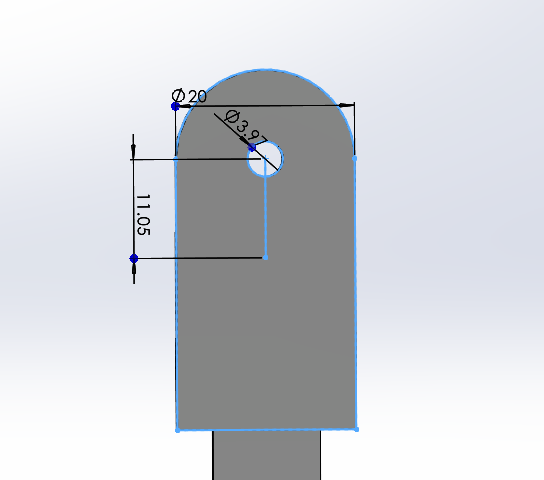
\includegraphics[width=\textwidth]{./../images/6-1-30}
        \caption{BASE草圖(3)}
        \label{fig:platform}
    \end{minipage}
    \hfill
    \begin{minipage}[b]{0.45\textwidth}
        \centering
        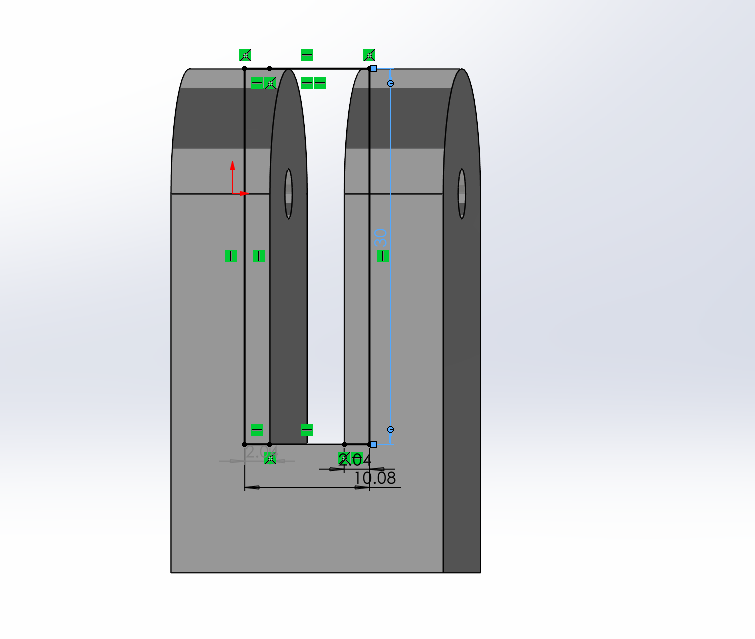
\includegraphics[width=\textwidth]{./../images/6-1-31} 
        \caption{BASE草圖(4)}
        \label{fig:feature1}
    \end{minipage}
\end{figure}


在距離方柱中心長 129mm 寬 25mm 處繪製一個長 31mm 寬 20mm 向上填料 7mm 的小平台用來定位馬達。

\begin{figure}[h!]
    \centering
    \begin{minipage}[b]{0.6\textwidth}
        \centering
        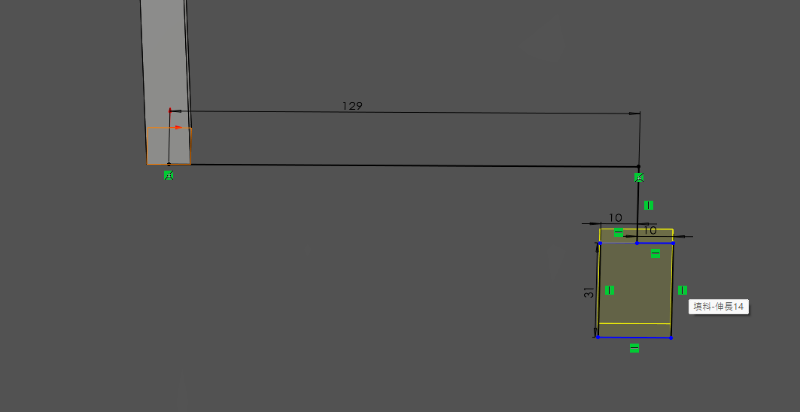
\includegraphics[width=\textwidth,height=0.30\textheight]{./../images/6-1-33}
        \caption{BASE草圖(5)}
        \label{fig:platform}
    \end{minipage}
    \hfill
    \begin{minipage}[b]{0.35\textwidth}
        \centering
        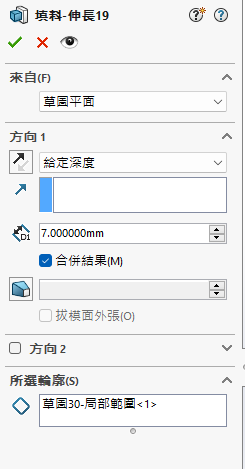
\includegraphics[width=\textwidth,height=0.35\textheight]{./../images/6-1-34} 
        \caption{編輯特徵(5)}
        \label{fig:feature1}
    \end{minipage}
\end{figure}

\newpage

並且在兩邊加畫底 15mm 高 45mm 的三角形支撐架防止馬達晃動。

\begin{figure}[htbp]
    \centering
    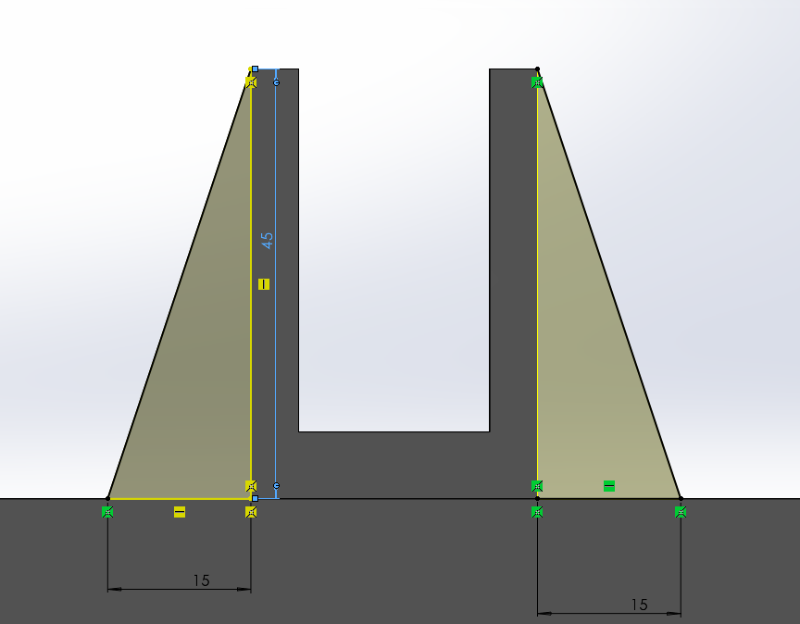
\includegraphics[width=0.70\textwidth]{./../images/6-1-35}
    \caption{BASE零件圖}
\end{figure}

第一版 base 完成圖。

\begin{figure}[htbp]
    \centering
    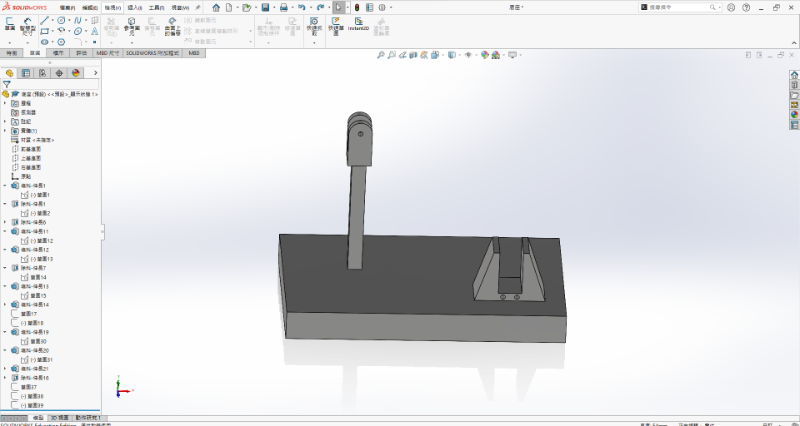
\includegraphics[width=0.9\textwidth]{./../images/6-1-36}
    \caption{BASE零件圖}
\end{figure}

\newpage

\textbf{修改部分}

底部去除浪費的部分改以長 165.6mm 圓直徑 22.35mm 的直狹槽代替。

\begin{figure}[htbp]
    \centering
    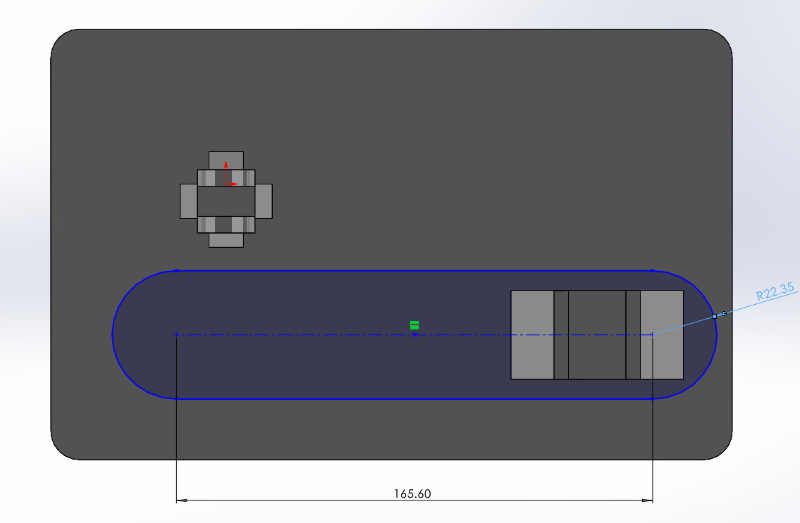
\includegraphics[width=0.85\textwidth]{./../images/6-1-37}
    \caption{修改BASE草圖(1)}
\end{figure}

為了好收納將左方柱子拔除留下一凹槽方便後續配合及螺絲孔。

\begin{figure}[htbp]
    \centering
    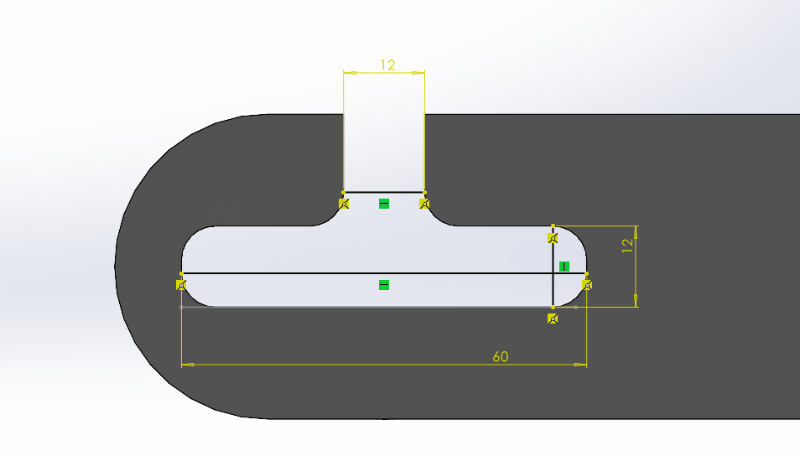
\includegraphics[width=0.85\textwidth]{./../images/6-1-38}
    \caption{修改BASE草圖(2)}
\end{figure}

\newpage

最終 base 完成圖。

\begin{figure}[htbp]
    \centering
    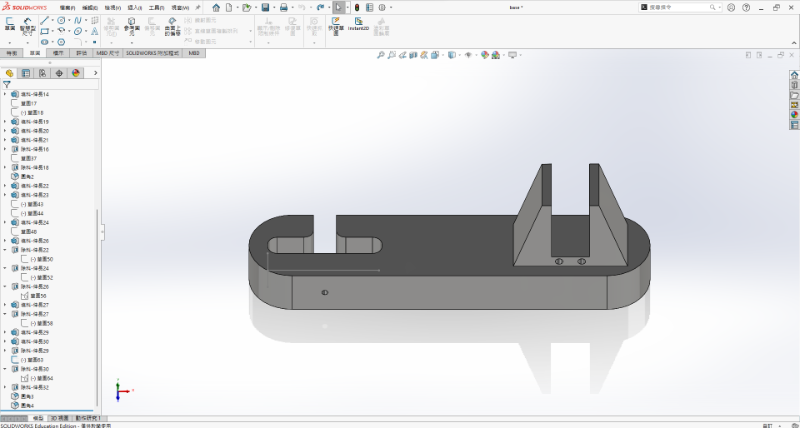
\includegraphics[width=0.9\textwidth]{./../images/6-1-39}
    \caption{最終BASE零件圖}
\end{figure}

\textbf{3D 列印成果}

\begin{figure}[htbp]
    \centering
    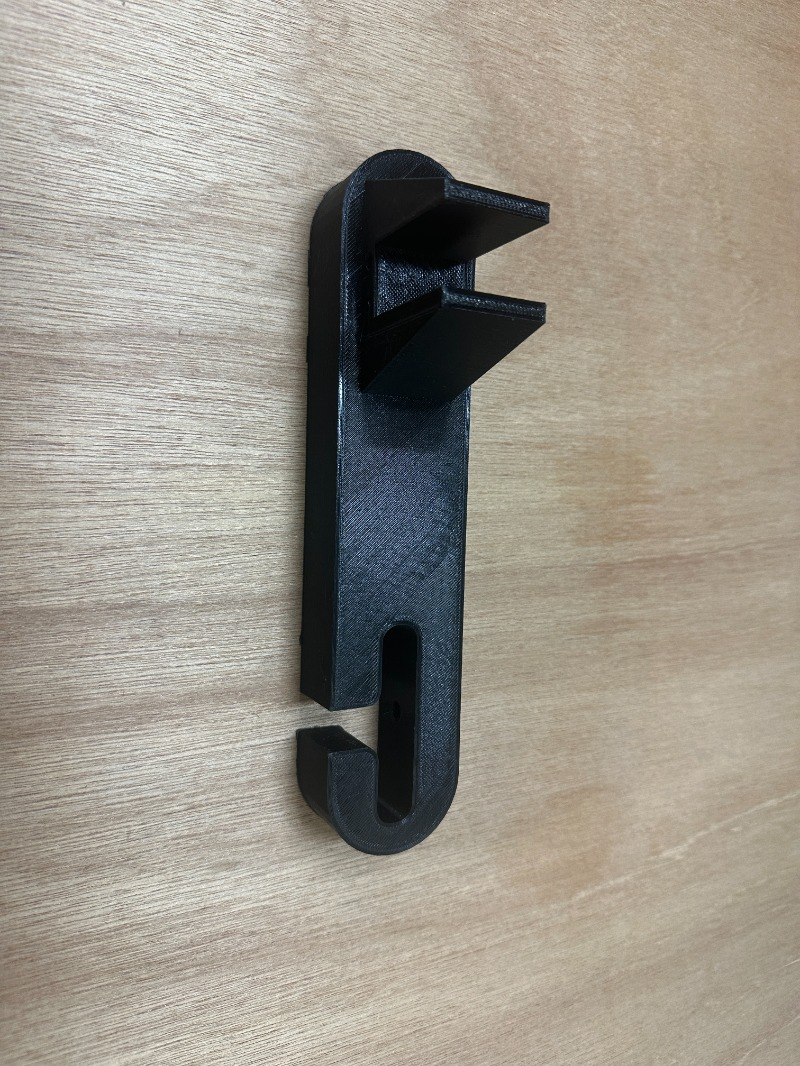
\includegraphics[width=0.45\textwidth]{./../images/6-1-25}
    \caption{BASE 3D列印完成圖}
\end{figure}

\newpage

\subsection*{support}

從底座拔除的部分目的好收納尺寸都沒有改變。
最終 support 完成圖。

\begin{figure}[htbp]
    \centering
    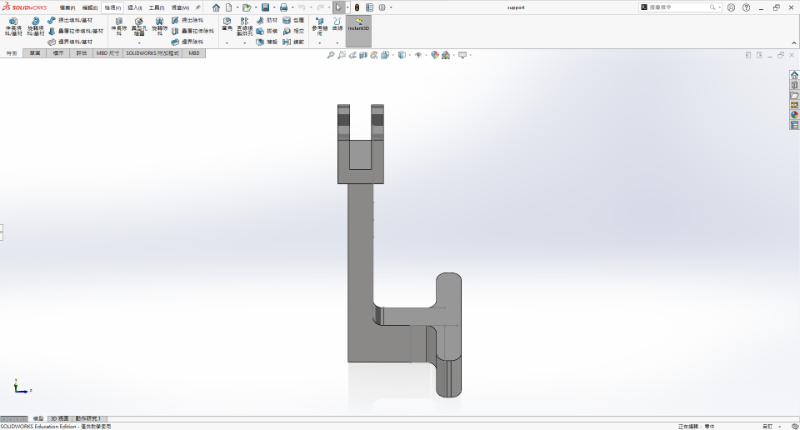
\includegraphics[width=0.90\textwidth]{./../images/6-1-40}
    \caption{最終SUPPORT零件圖}
\end{figure}

\textbf{3D 列印成果}

\begin{figure}[htbp]
    \centering
    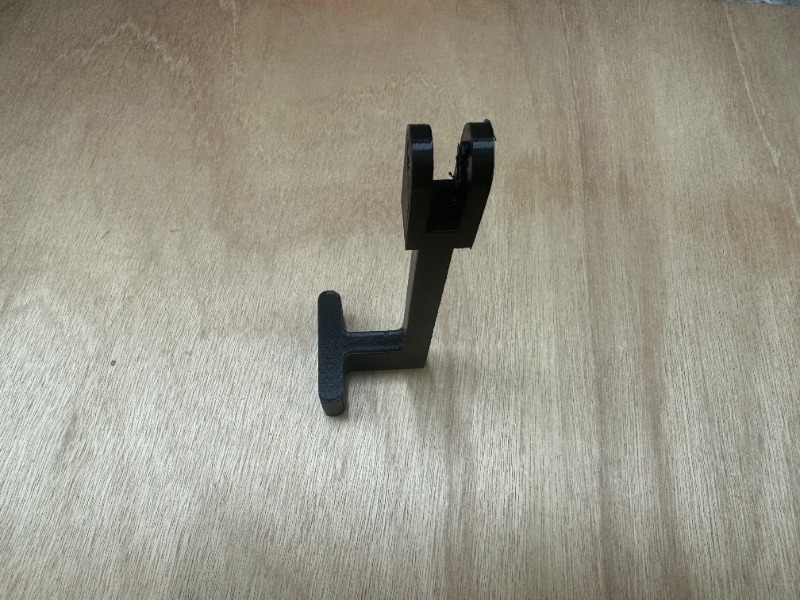
\includegraphics[width=0.80\textwidth]{./../images/6-1-24}
    \caption{SUPPORT 3D列印完成圖}
\end{figure}

\subsection*{link}

上方連結處與 support 尺寸一致皆為長 30.28mm 寬 20 的長方體然後在長方體上畫直徑 20mm 的半圓最後在圓的中心繪製一個 3.98mm 的小孔最後在長方體上畫一個長 30mm 寬 10.8mm 的小長方體伸長除料選擇完全貫穿方便與上方 platform 配合。

\begin{figure}[htbp]
    \centering
    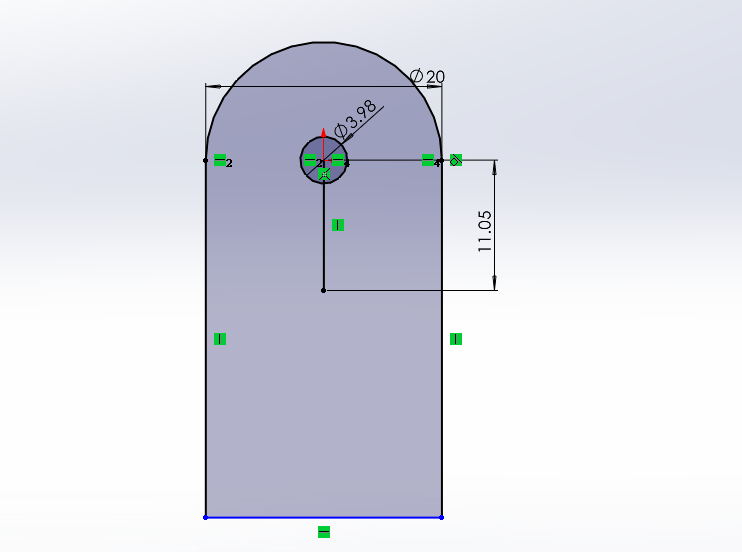
\includegraphics[width=0.5\textwidth]{./../images/6-1-41}
    \caption{LINK草圖(1)}
\end{figure}

下方為 12mm $\times$ 12mm 的方柱並填料 68mm 方便與馬達進行配合。

\begin{figure}[h!]
    \centering
    \begin{minipage}[b]{0.6\textwidth}
        \centering
        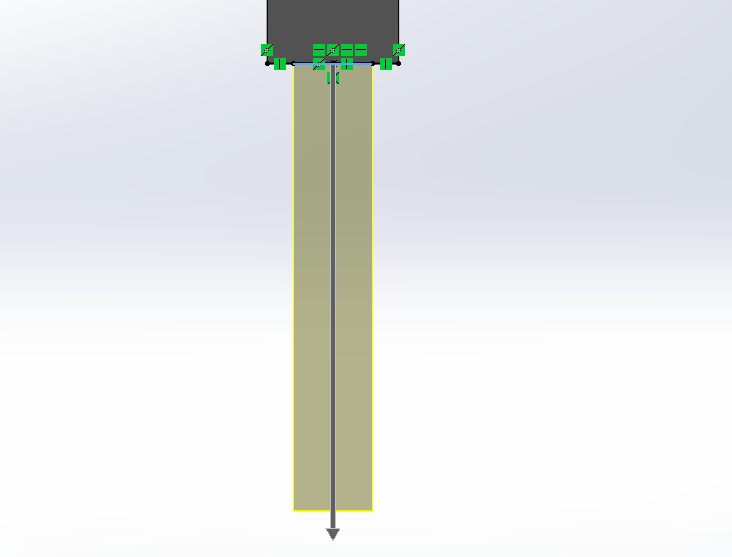
\includegraphics[width=\textwidth,height=0.30\textheight]{./../images/6-1-42}
        \caption{LINK草圖(2)}
        \label{fig:platform}
    \end{minipage}
    \hfill
    \begin{minipage}[b]{0.35\textwidth}
        \centering
        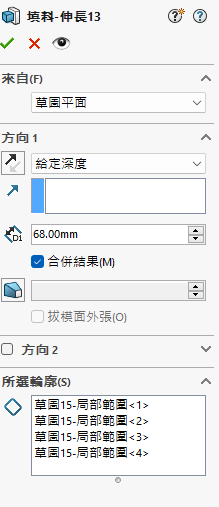
\includegraphics[width=\textwidth,height=0.35\textheight]{./../images/6-1-43} 
        \caption{編輯特徵(6)}
        \label{fig:feature1}
    \end{minipage}
\end{figure}

\newpage

最終 link 完成圖。

\begin{figure}[htbp]
    \centering
    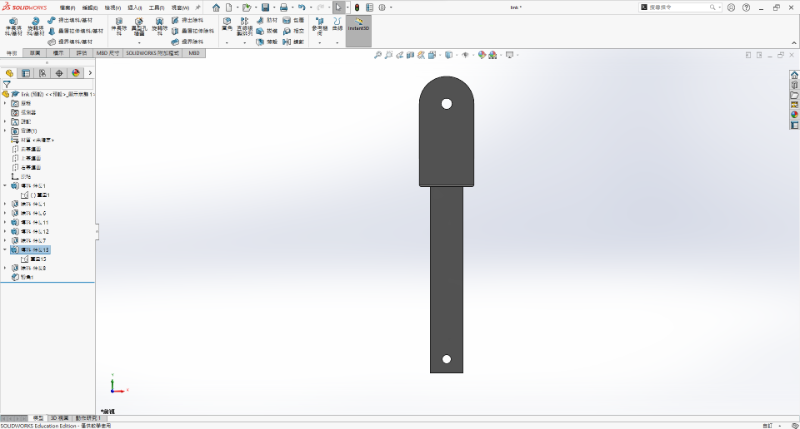
\includegraphics[width=0.85\textwidth]{./../images/6-1-44}
    \caption{最終LINK零件圖}
\end{figure}

\textbf{3D 列印成果}

\begin{figure}[htbp]
    \centering
    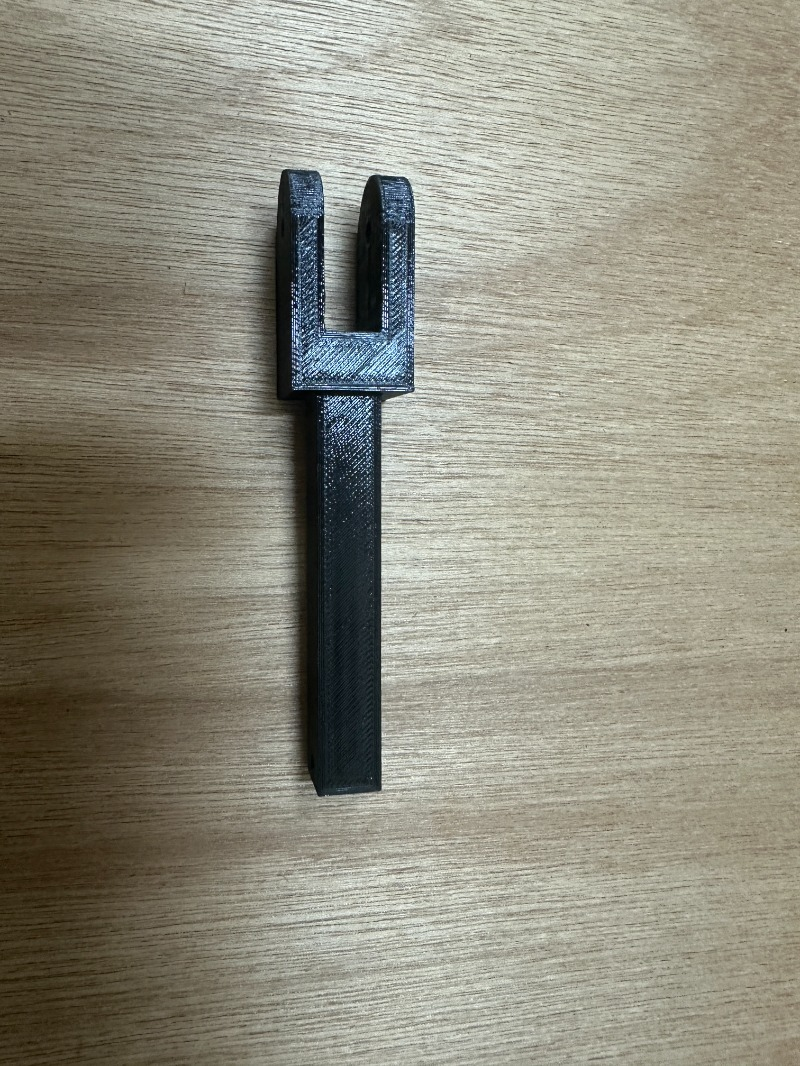
\includegraphics[width=0.46\textwidth]{./../images/6-1-23}
    \caption{LINK 3D列印完成圖}
\end{figure}

\newpage

\subsection*{crank}

畫一個長36mm寬5mm的crank填料3mm並留兩個3.2mm的圓孔方便鎖上螺栓配合base與link


\begin{figure}[h!]
    \centering
    \begin{minipage}[b]{0.6\textwidth}
        \centering
        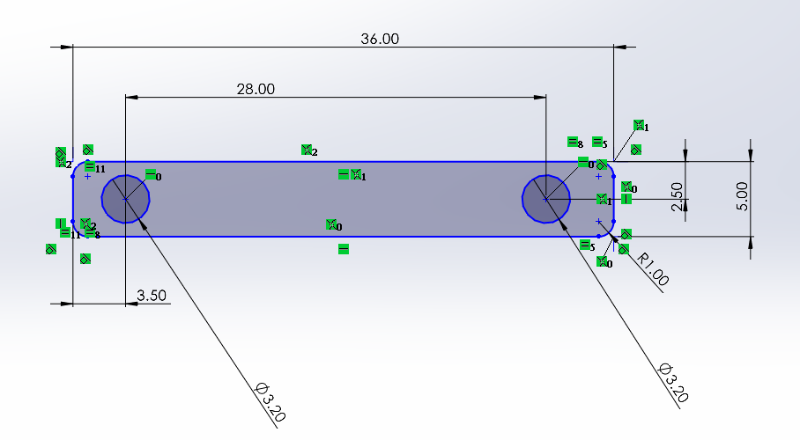
\includegraphics[width=\textwidth,height=0.30\textheight]{./../images/螢幕擷取畫面 2024-05-25 220448}
        \caption{crank草圖(1)}
        \label{fig:platform}
    \end{minipage}
    \hfill
    \begin{minipage}[b]{0.35\textwidth}
        \centering
        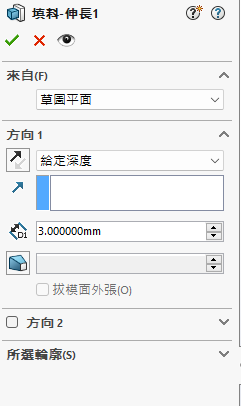
\includegraphics[width=\textwidth,height=0.35\textheight]{./../images/螢幕擷取畫面 2024-05-25 221952} 
        \caption{編輯特徵(7)}
        \label{fig:feature1}
    \end{minipage}
\end{figure}

最終crank完成圖

\begin{figure}[htbp]
    \centering
    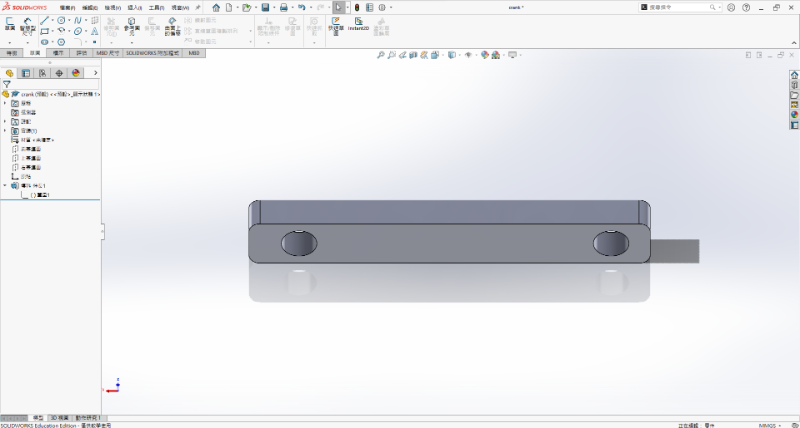
\includegraphics[width=1\textwidth]{./../images/螢幕擷取畫面 2024-05-25 230501}
    \caption{baffle草圖(1)}
\end{figure}

\newpage

\subsection*{baffle}

繪製一個配合platform,兩兩相組合的檔塊,透過螺絲逼緊的方式夾緊於platform,保留可調整位置、可拆除的特性,以輔助調整控制參數,如此一來當參數錯誤時,球不會直接飛離平台。而上方的拱型則是避免干擾到雷射感測器的訊號。

\begin{figure}[htbp]
    \centering
    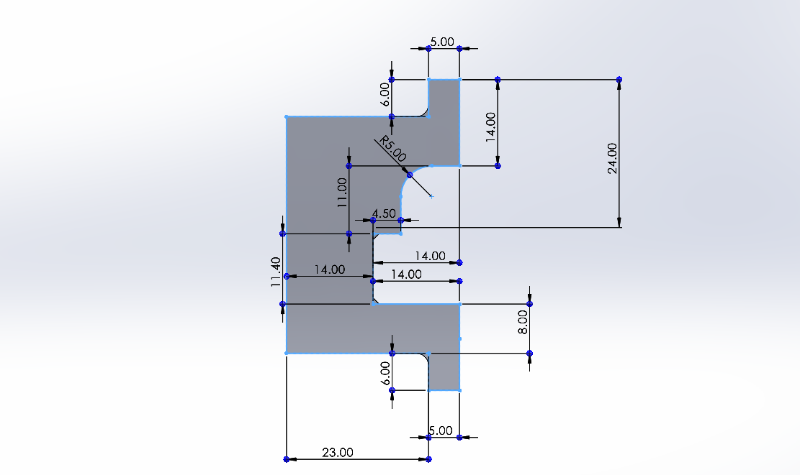
\includegraphics[width=1\textwidth]{./../images/螢幕擷取畫面 2024-05-25 224335}
    \caption{baffle草圖(1)}
\end{figure}

最終baffle完成圖

\begin{figure}[htbp]
    \centering
    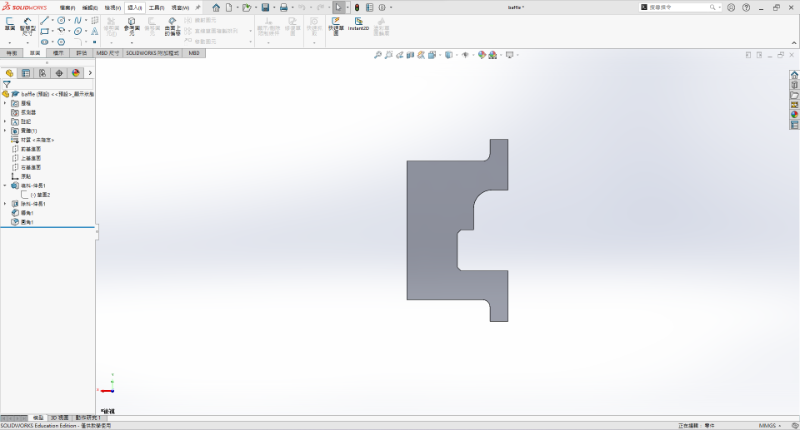
\includegraphics[width=1\textwidth]{./../images/螢幕擷取畫面 2024-05-25 230234}
    \caption{baffle草圖(1)}
\end{figure}

\subsection*{assemble}

組合完成圖。

\begin{figure}[htbp]
    \centering
    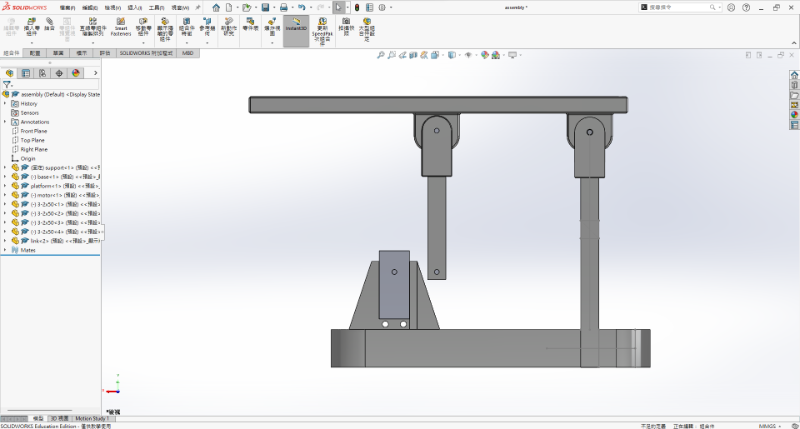
\includegraphics[width=1\textwidth]{./../images/6-1-45}
    \caption{ASSEMBLE組合圖(1)}
\end{figure}

\begin{figure}[htbp]
    \centering
    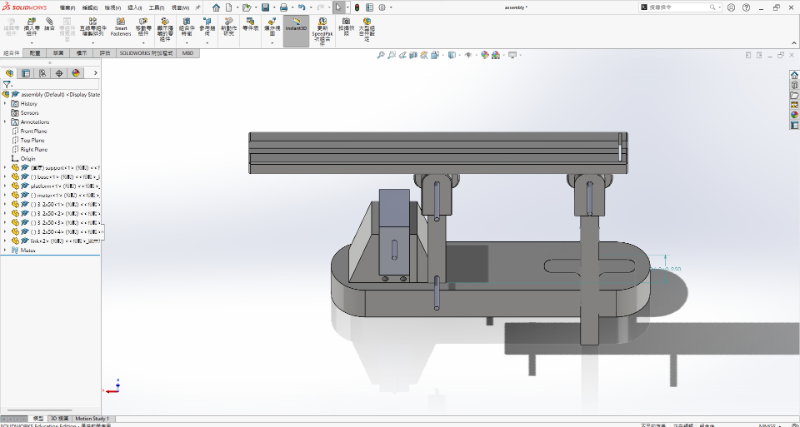
\includegraphics[width=1\textwidth]{./../images/6-1-46}
    \caption{ASSEMBLE組合圖(2)}
\end{figure}


\subsection*{驅動方式}

使用金屬齒輪伺服馬達配合程式控制平台,程式放置於 6-3。

